\documentclass{report}

\usepackage{ugentstyle}
\usepackage{listings}


\begin{document}
	\maketitle{Gedistribueerde toepassingen}
    \tableofcontents

	
	\part{Theorie}
	\chapter{Extensible Stylesheet Language Family}
	\section{Inleiding}
	XSL staat voor \textit{Extensible Stylesheet Language Family} en is een standaard om XML-documenten te presenteren en te transformeren. De drie componenten van XSL zijn:
	\begin{itemize}
		\item \textbf{XSLT} (Extensible Stylesheet Language Transformations) : dit is een XML-taal dat XML-documenten kan omvormen naar opnieuw XML, maar kan ook HTML, \LaTeX, JSON, enz... zijn.
		\item \textbf{XPath} : dit is een taal dat waarmee bepaalde stukken van een XML-document kunnen gemanipuleerd worden aan de hand van het opbouwen van paden.
		\item XSL-FO (XSL Formatting Objects)
	\end{itemize}
	\section{XSLT}
	\subsection{Structuur}
	Een XSLT-bestand moet altijd voldoen aan volgende structuur:
	\begin{lstlisting}
<?xml version="1.0" encoding="UTF-8"?>
<xsl:stylesheet version="1.0" 
	xmlns:xsl="http://www.w3.org/1999/XSL/Transform">
	<xsl:output method="html"/>
	<xsl:template match="patroon">
	...
	</xsl:template>
	...
</xsl:stylesheet>
	\end{lstlisting}
	\begin{enumerate}
		\item \texttt{xsl:stylesheet} is het basiselement
		\item \texttt{xsl:output} is het element dat het type transformatie vastlegt in het attribuut \textit{method}
		\item \texttt{xsl:template} bevat wat er moet gebeuren voor elk element dat aan \textit{patroon} voldoet.
	\end{enumerate}

	\subsection{Instructie-elementen}
	\begin{itemize}
		\item \textbf{xsl:value-of} : Bepaalt de waarde van een XPath uitdrukking.
		
			  \texttt{<xsl:value-of select='uitdrukking'/>}
			  
		\item \textbf{apply-templates} : Zal de templates van de onmiddelijke kindelementen van het huidig element toepassen. Indien er geen templates zijn, zal de inhoud van het element naar de uitvoer uitgeschreven worden. Het optionele \textit{select} attribuut zal enkel de templates uitvoeren voor elk element die aan de uitdrukking voldoet.
		
			  \texttt{<xsl:apply-templates [select='uitdrukking']/>}
			  
		\item \textbf{xsl:for-each} : Voert een actie uit voor alle knopen die door het \textit{select}-attribuut bepaalt wordt. Binnen de for-each kunnen meerdere instructie-elementen voorkomen.
		
			  \texttt{<xsl:for-each select'uitdukking'>...</xsl:for-each>}
			  
		\item \textbf{xsl:sort} :Dit is een kindelement van \textit{xsl:apply-templates} of een \textit{xsl:for-each} element. Dit element zal de knopen sorteren die aan de waarde van het select attribuut voldoen. Optionele attributen zijn
			\begin{itemize}
				\item data-type : legt het datatype vast (\textit{text} of \textit{number}). Dit heeft een invloed op de sorteervolgorde (bij \textit{text} is 10 kleiner dan 2).
				\item order : bepaalt de sorteervolgorde (\textit{ascending} of \textit{descending}).
			\end{itemize}
				
				\texttt{<xsl:sort select='uitdrukking' [data-type='text|number'] [order='ascending|descending]/>}
		
		\item \textbf{xsl:if} : Dit is een typische selectiestructuur. Het bevat als enig attribuut \textit{test} met als waarde een predicaat.
		
			  \texttt{<xsl:if test='logische uitdrukking'> ... </xsl:if>}
			  
		\item \textbf{xsl:choose} : Een alternatieve selectiestructuur equivalent zoals een switch in programeertalen zoals Java en C\#. Dit element wordt gevolgd door één of meerdere \textbf{xsl:when} elementen. Een xsl:when element is equivalent met een xsl:if element en heeft ook als enig attribuut \textit{test}.
		\begin{lstlisting}
<xsl:choose>
	<xsl:when test="logische uitdrukking 1">
		... 
	</xsl:when>
	<xsl:when test="logische uitdrukking 2"> 
		... 
	</xsl:when>
	...
</xsl:choose>
		\end{lstlisting}
		
		\item \textbf{xsl:text} : Wanneer tekst spaties bevat is het aan te raden om xsl:text te gebruiken zodat deze ook opgenomen worden in het resultaat. Spaties die niet in een xsl:text element staan worden genegeerd.
		
		\texttt{<xsl:text>stukje tekst</xsl:text>}
		
		\item \textbf{xsl:variable} : Legt een constante variabele vast. Het verplichte attribuut is \textit{name}, wat de naam van de variabele vastlegt. Het invullen van deze waarden kan op twee manieren :
		\begin{enumerate}
			\item via het select attribuut \texttt{<xsl:variabele name='varnaam' select='uitdrukking'/>}
			\item via de inhoud van het element: \texttt{<xsl:variabele name ="varnaam">
				...
			</xsl:variable>}
			In dit geval kan de waarde ook opgebouwd worden uit meerdere instructies.
		\end{enumerate}
	
		\item \textbf{xsl:param} : Indien dit element gedeclareerd wordt in het begin van een xls:template element, dan is het mogelijk om parameters mee te geven aan dit template. De declaratie kan op dezelfde manier gebeuren als bij xsl:variabele.
		
		\item \textbf{xsl:with-param} : Dit element is een kindobject van xsl:apply-templates. Dit element vult voor een bepaalde \textit{name} de waarde die in \textit{select} staat.
		
		\begin{lstlisting}
<xsl:apply-templates ...>
	<xsl:with-param name='varnaam' select='uitdrukking'>
</xsl:apply-templates>
		\end{lstlisting} 
	\end{itemize}

	\chapter{XML Path Language (XPath)}
	XPath is een taal om knopen te selecteren van een XML-document. Het resultaat van een XPath-uitdrukking kan een getal, string of logische waarde zijn.
	\section{Paden}
	Belangrijke XPath uitdrukkingen zijn paden. Een pad identificeert nul, één of meerdere knopen in een XML-document. Een pad bestaat uit \textit{location steps} die verbonden zijn met een /. Bij elk pad zijn volgende wildcards mogelijk:
	\begin{itemize}
		\item *: selecteert elk elementknoop in de huidige context.
		\item node(): selecteert alle knopen, dus niet enkel elementen
		\item @*: selecteert alle attributen in de huidige context.
	\end{itemize}
	\subsection{Basispad (Root Location Path)}
	
	Het eenvoudigste pad is \texttt{/} en selecteert het root-element van het XML-document. Verder is dit een absoluut pad, dus deze uitdrukking zal \textbf{altijd} het root-element teruggeven.
	\subsection{Kinelement-stap (Child Element Location Steps)}
	Dit pad bestaat uit de naam van een element en selecteert alle elementen met deze naam in de huidige context. De context is afhankelijk van de ouder. 
	
	\begin{lstlisting}
<xsl:template match ="author">
	<xls:apply-templates select="name" />
</xls:template>
	\end{lstlisting}
	In dit voorbeeld wordt de XPath uitdrukking van het selectattribuut \texttt{/author/name/}.
	
	\subsection{Attribuut-stap (Attribute Location Steps)}
	Een attribuut selecteren begint met een @ en wordt gevolgd door de naam van het attribuut.	
	\begin{lstlisting}
<xsl:template match ="query">
	<xls:value-of select="@isbn"/>
</xls:template>
	\end{lstlisting}
	
	\subsection{Voorwaarden}
	\begin{lstlisting}
<xsl:apply-templates select="//book[title='XML']//name[.='Ongenae]"/>
	
<xsl:apply-templates select="//person[@born<=1976]"/>
	\end{lstlisting}
	\subsection{Lange padnamen}
	In elke XPath uitdrukking wordt elke stap voorafgegaan door de child:: as.
	
	\texttt{books/book/isbn => child::books/child::book/child::isbn}
	
	andere assen:
	\begin{itemize}
		\item parent (of ..)
		\item self (of .)
		\item descendant-or-self (of //)
		\item ancestor 
		\item ancestor-or-self
		\item namespace
		\item descendant
		\item following-sibling
		\item preceding-sibling
		\item following
		\item preceding
	\end{itemize}
	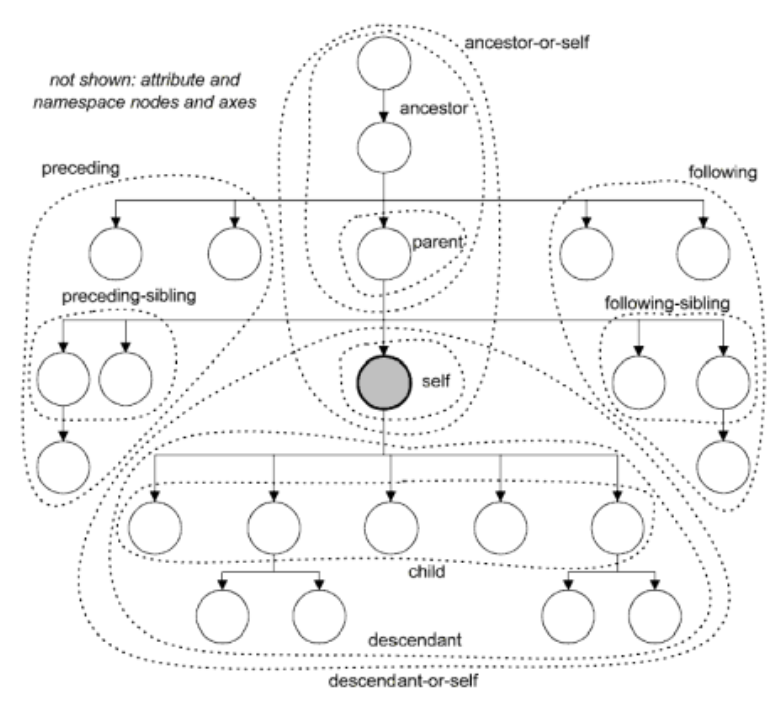
\includegraphics[width=\textwidth]{assen_XPath}
	
	\section{Andere XPath-uitdrukkingen}
	XPath kan ook getallen, logische waarden en strings manipuleren.
	\subsection{Datatypes}
	\begin{itemize}
		\item \textbf{Getallen} : Stel dat \textit{born} het geboortejaar van een persoon is, dan zal de volgende uitdrukking de eeuw uitschrijven van dit jaar.
		\texttt{<xls:value of select="(@born - (@born mod 100)) div 100 + 1"}
		
		\item \textbf{Strings} : Strings staan tussen enkele of dubbele aanhalingstekens. Strings vergelijken kan met = en != operatoren.
		
		\item \textbf{Logische waarden} : De sleutelwoorden true en false bestaan niet in XPath, wel worden ze respectievelijk voorgesteld door de functies true() en false(). Op logische waarden kunnen de operatoren \textit{and} en \textit{or} toegepast worden. Met not(...) wordt de negatie toegepast.
		
	\end{itemize}

	\section{Functies}
	XPath kent een aantal functies.
	\begin{itemize}
		\item \textbf{Knopenfuncties} zoals \textit{position()}, \textit{last()}, \textit{count(...)} en \textit{id(...)} bepalen respectievelijk \begin{itemize}
			\item het volgnummer van de huidige knoop in de context, 
			\item het aantal knopen in de huidige context (volgnummer van de laatste knoop),
			\item telt het aantal knopen van het argument, dat een verzameling knopen is en
			\item bepaalt een verzameling knopen. Deze verzameling bevat alle elementen van een XML-document met één van de gespecifieerde ID's. Het argument is een string bestaande uit ID's gescheiden door spaties.
		\end{itemize}
	
		\item \textbf{Stringfuncties} zoals \textit{concat(...)}, \textit{contains(...)}, \textit{starts-with(...)}, \textit{string(...)} (conversie naar string) en \textit{string-length(...)}.
		
		\item \textbf{Logische functies} zoals \textit{true()}, \textit{false()}, \textit{not(...)}, \textit{boolean(...)} (conversie naar bool waarde).
		
		\item \textbf{Numerieke functies} zoals \textit{ceiling(...)}, \textit{floor(...)}, \textit{number(...)}, \textit{round(...}).
	\end{itemize}

\chapter{Webservices}
Een gedistribueerd systeem zal over verschillende servers API's beschikbaar hebben. Tabel \ref{table:mono_vs_distributed} geeft de voornaamste verschillen tussen een monolitische architectuur en een gedistribueerde architectuur.
\begin{table}[h]
	\begin{tabular}{l | l | l}
		& Monolitisch & Gedistribueerd \\
		\hline
		Communicatie & Tussen processen, gedeeld geheugen & Over een netwerk \\
		Globale toestand & Mogelijk & Niet mogelijk \\
		Globale tijd & Mogelijk via lokaal besturingssysteem & Niet mogelijk \\
		Fouten & Eenvoudig te ontdekken & Gedeeltelijk falen moeilijk te ontdekken \\
		Locatie & Alle componenten op één machine & Variabel \\
		Beveiliging & Taak van het besturingssysteem & Inherent kwetsbaar door networkcommunicatie.
	\end{tabular}
	\label{table:mono_vs_distributed}
\end{table}
Er zijn twee belangrijke componenten bij gedistribueerde systemen, \textbf{EDI  (Electronic Data Interchange)} en \textbf{RPC (Remote Procedure Call)}.
 
\section{Componenten}
\subsection{EDI}
Dit soort toepassingen digitaliseren het papierwerk dat vaak plaatsvindt in eender welke organisatie. Dit werkt in drie stappen:
\begin{enumerate}
	\item Verzamel de informatie die verzonden moet worden. Deze data komt vaak uit interne bronnen, die een willekeurige structuur kunnnen hebben?
	\item Zet deze informatie om naar het EDI formaat door gebruik te maken van vertaler die de interne informatie kan omzetten naar het EDI formaat.
	\item Verstuur deze informatie naar de bestemmeling. Een zender en ontvanger zijn direct aangesloten met elkaar via software.
\end{enumerate}

\subsection{RPC}
RPC is het aanroepen van een procedure (functie, methode, ...) op een ander toestel dan waarop een programma fysiek uitgevoerd wordt. Dit proces bevat volgende stappen:
\begin{enumerate}
	\item De client maakt een RPC aan en verstuurt deze naar een server die deze call can behandelen.
	\item De server verwerkt de procedure en stuurt het resultaat terug naar de client.
	\item De client kan gebruik maken van dit resultaat op lokaal niveau.
\end{enumerate}
\section{Gedistribueerde objectsystemen}
Gedistribueerde systemen maken gebruik van EDI en RPC om een systeem te implementeren. Er worden enkele besproken zoals \textbf{RMI (Remote Method Invocation)}, \textbf{DCOM (Distributed Component Object Model)} en \textbf{CORBA (Common Object Request Broker Architecture)}
\subsection{RMI}
Deze technologie is ontwikkelt door Oracle en bestaat typisch uit een \textbf{Server} en \textbf{Client} applicatie. Een server zal methoden beschikbaar stellen en zal wachten tot dat een client deze methode uitvoert (invocation). RMI is het mechanisme dat de verbinding en informatieuitwisseling tussen een client en een server behandelt. Een gedistribueerd systeem gebasseerd op RMI kan de volgende 3 zaken uitvoeren.
\begin{enumerate}
	\item \textit{Lokalisatie van remote objecten.} Remote objecten moeten opgeslagen worden in een zogenaamde \textbf{RMI registery}.
	\item \textit{Communicatie met remote objecten.} Het aanroepen van methoden van een remote object wordt volledig door RMI behandelt. Dit heeft als gevolg dat een programmeur niet eens moet weten dat hij met een remote object bezig is.
	\item \textit{Klassedefinities laden van remote objecten.} Aangezien dat RMI objecten kan terugsturen/versturen, voorziet RMI de mogelijkheid om klassedefinities van deze objecten op te halen.
\end{enumerate}
\subsection{DCOM}
DCOM is een uitbreiding op COM om communicatie tussen verschillende toestellen, hetzij op een LAN, hetzij op een WAN of zelfs op het internet aan te spreken. DCOM behandelt het low-level gedeelte van de netwerkcommunicatie, zodat een programmeur hier zich niet meer mee bezig hoeft te houden.  
\subsection{CORBA}
CORBA is zoals de anderen, ook een manier om communicatie te hebben tussen verschillende systemen. CORBA baseert zich op 4 punten:
\begin{enumerate}
	\item Applicatieobjecten die specifiek zijn voor de applicatie. Een CORBA object is een encapsulatie van zulke objecten.
	\item Een \textbf{ORB (Object Request Broker)} dat de requests van verschillende services behandelt. 
	\item Een verzameling van services die waarschijnlijk gebruikt zullen worden door veel applicaties. 
	\item Een verzameling van componenten die bovenop deze services gebouwd zijn.
\end{enumerate} 


\section{MOM}
\textbf{MOM (Message Oriented Middleware)} is een software systeem dat instaat voor het aanmaken, versturen, ontvangen en lezen van berichten op zowel synchrone of aysnchrone manier. Een client applicatie moet dus enkel deze middleware aanspreken om berichten op te halen of te versturen.

\section{SOA}
\textbf{SOA (Service Oriented Architecture)} is een architectuurstijl dat gebruik maakt van services die onafhankelijk zijn van andere services. Een service kan individueel aangepast worden zonder dat andere services hiervan last hebben. Deze architectuurstijl kent een aantal uitdagingen:
\begin{itemize}
	\item Gelijktijdige toegang tot bronnen
	\item Wat indien een deel van de opdracht mislukt?
	\item Wat als één partner incompatibel wordt?
	\item Geen gedeeld geheugen voor requester en provider
	\item Traagheid en onbetrouwbaarheid gebruike transport
\end{itemize}
Er blijkt ook een gelijkheid te zijn met SOA en microservices. Het verschil tussen microservices en SOA is 
\todo{saai}

\section{Webservices in Java}
Voor webservices te implementeren in java maken we gebruik van SOAP. Een SOAP aanvraag ziet er als volgt uit :
\begin{lstlisting}
<?xml version="1.0" encouding="UTF-8"?>
<S:Envelope 
  xmlns:S="http://schemas.xmlsoap.org/soap/envelope/">
  <S:Header/>
  <S:Body>
    <ns2:geefBoek xmlns:ns2="http://web.boeken.iii.be/">
      <isbn>isbn2</isbn>
    </ns2:geefBoek>
  </S:Body>
</S:Envelope>
\end{lstlisting}

Een eenvoudige webserivce dat een boek opvraagd met een bepaald isbn ziet er dan zo uit:
\begin{lstlisting}
@WebService(serviceName = "Catalogus")
public class Catalogus {
  @WebMethod(operationName = "geefBoek")
  public Boek geefBoek(@WebParam(name = "isbn") String isbn){
    try {
      BoekenLijst boeken = new BoekenLijstImpl();
      return boeken.geefBoek(isbn);
    } catch(Exception e) {
      return null;
    }
  }
}
\end{lstlisting}
\section{Webservices in C\#}
\todo{al de rest lel}

\chapter{Netwerkprogrammatie in Java}
Belangrijke netwerkklassen in java, in de package \underline{\texttt{java.net}}:
\begin{itemize}
    \item \textbf{TCP} 
        \begin{itemize}
            \item URL
            \item URLConnection
            \item Socket
            \item ServerSocket
        \end{itemize}
    \item \textbf{UDP}
        \begin{itemize}
            \item DatagramPacket
            \item DatagramSocket
            \item MulticastSocket
        \end{itemize}
\end{itemize}

De cliënt maakt een \texttt{Socket} object aan. De constructor heeft de locatie van een bepaalde server, en een poortnummer, die de server openzet. Communicatie met de socket gebeurt met de \texttt{PrintWriter} klasse, die naar de server zal sturen, en de \texttt{BufferedReader} klasse, die berichten van de server zal ontvangen. Gebruik best de try met resources om instanties van deze objecten te maken, zodat ze automatisch verdwijnen indien de code uit het \texttt{try} block komt. Vanaf dan kan er met de server gecommuniceert worden door weg te schrijven via de \texttt{PrintWriter}. Wachten op een bericht van de server kan door de \texttt{readLine()} methode van de \texttt{BufferedReader}klasse op te roepen. Dit is een synchrone methode dus de applicatie zal blokkeren. 

De server zal gebruik maken van een \texttt{ServerSocket} klasse. Deze werkt op identiek dezelfde manier als de \texttt{Socket} klasse die de cliënt gebruik, behalve dat een \texttt{ServerSocket} klasse meerdere sockets kan accepteren. Tot slot is er nog een \underline{protocol} nodig, die de communicatie tussen de server en communicatie beschrijft. Een eenvoudig protocol vereist bijvoorbeeld dat een bericht start met een bepaald sleutelwoord.

\begin{lstlisting}
// CLIENT
String hostName = "localhost";
int portNumber = 4444;
try(
    Socket socket = new Socket(hostName, portNumber);
    PrintWriter out = new PrintWriter(socket.getOutputStream(), true);
    BufferedReader in = new BufferedReader(
        new InputStreamReader(socket.getInputStream())
    );
){
    String input = ... // input ophalen van gebruiker
    while(!input.equals("exit")){
        out.println(input); // naar server
        System.out.println("echo: ) + in.readLine()); // van server
        input = ... // input ophalen van gebruiker
    }
} catch (IOException ex) {
    System.err.println(ex.getMessage());
}

// SERVER
try {
    ServerSocket socket = new ServerSocket(4444);
    while(true) {
        try(
            PrintWriter out = new PrintWriter(
                socket.getOutputStream(), true
            );
            BufferedReader in = new BuffereadReader(
                new InputStream(socket.getInputStream())
            );
        ){
            String input, output;
            while((input = in.readLine()) != null){
                output = protocol.processInput(input);
                out.println(output);
                if(output.equals("Bye")){
                    break;
                }
            }
        }
    }
}
\end{lstlisting}

Een socket wordt best geïmplementeerd met behulp van threads, zodat verschillende cliënts op hetzelfde moment behandeld kunnen worden.

\chapter{Java NIO}
Java NIO (New IO) biedt een alternatieve manier om met IO te werken.
\begin{itemize}
    \item \textbf{Channels en Buffers.} Data wordt altijd gelezen van een bepaald kanaal naar een buffer, of geschreven van een buffer naar een kanaal.
    \item \textbf{Non-blocking IO.} Een thread kan aan een kanaal vragen om data van een buffer in te lezen. Terwijl het kanaal dit doet, kan de thread andere zaken uitvoeren en wachten tot het kanaal klaar is.
    \item \textbf{Selectors.} Een selector is een object that meerdere kanalen kan monitoren. Het reageert op events (connectie opened, data arrived, ...). Een enkele thread kan meedere kanalen monitoren met behulp van selectors. Een selector registreren gebeurt door een kanaal mee te geven, en de \texttt{select()} methode op te roepen van de \texttt{Selector} klasse.
\end{itemize}
De kern van Java NIO zijn de klassen \texttt{Channel}, \texttt{Buffer} en \texttt{Selector}. Andere klassen zoals \texttt{Pipe} en \texttt{FileLock} dienen gebruikt te worden in samenwerking met de drie kernklassen. Elke klasse kent meerdere implementaties. Zo kent de \texttt{Channel} klasse bijvoorbeeld: \texttt{FileChannel}, \texttt{DatagramChannel}, \texttt{SocketChannel} en \texttt{ServerSocketChannel}. De klasse \texttt{Buffer} kent meerdere implementies afhankelijk van het datatype: \texttt{ByteBuffer}, \texttt{CharBuffer}, \texttt{DoubleBuffer}, \texttt{FloatBuffer}, \texttt{IntBuffer}, \texttt{LongBuffer}, \texttt{ShortBuffer}. 
De verschillen tussen de \texttt{Channel} en \texttt{Stream} klasse zijn:
\begin{itemize}
    \item Lezen en schrijven is mogelijk met één kanaal. Een stream is ofwel leesmode of schrijfmode.
    \item De lees en schrijfoperatie kan asynchroon gebeuren.
    \item Een kanaal kan lezen van, of schrijven naar een Buffer
\end{itemize}
Het gebruik van een eenvoudig \texttt{Channel} object:
\begin{lstlisting}
RandomAccessFile file = new RandomAccessFile("data/file.txt", "rw");
FileChannel inChannel = file.getChannel();
ByteBuffer buffer = ByteBuffer.allocate(48);
int bytesRead = inChannel.read(buf);
while(bytesRead != -1){
    System.out.println("Read " + bytesRead);
    buf.flip();
    while(buf.hasRemaining()){
        System.out.print((char) buf.get());
    }
    buf.clear();
    bytesRead = inChannel.read(buf):
}
file.close();
\end{lstlisting}
De flip methode van een een buffer zal van de mode van lezen naar schrijven omzetten, of omgekeerd.


\end{document}